\documentclass[11pt]{article}

\usepackage{amsmath}
\usepackage[a4paper, margin=0.5in]{geometry}
\usepackage{graphicx} % daj an 1in jak chcesz normalniejszy margines, ale kod mi się w linii nie mieści :P
\usepackage[utf8]{inputenc}
\usepackage[T1]{fontenc}
\usepackage[polish]{babel}
\usepackage{float}
\usepackage{hyperref}
\usepackage{cleveref}
\usepackage{subfigure}

\title{Zadanie 6. Własna metoda i testy globalnej wypukłości}
\author{Oskar Kiliańczyk 151863 \& Wojciech Kot 151879}
\date{}

\begin{document}

\maketitle
\newpage

\section{Opis zadania}\label{sec:opis-zadania}
Zadanie polega na wygenerowaniu losowo 1000 optimów lokalnych, za pomocą zachłannej wersji przeszukiwania lokalnego,
oraz bardzo dobrego rozwiązania za pomocą najlepszej do tej pory metody.
Tą metodą powinna być własna metoda, której opracowanie również jest częścią tego zadania.
Następnie dla każdego z lokalnych optimów należy obliczyć podobieństwo do rozwiązania referencyjnego oraz średnie podobieństwo do poozstałych optimów lokalnych ze zbioru, oraz współczynnik korelacji.
Stosowane miary podobieństwa to:
\begin{enumerate}
    \item Liczba par wierzchołków przydzielonych w obu rozwiązaniach razem do jednego cyklu
    \item Liczba wspólnych par krawędzi
\end{enumerate}


\section{Własna Metoda}\label{sec:wasna-metoda}

\subsection{Pierwsza heurystyka konstrukcyjna}\label{subsec:pierwsza-heurystyka-konstukcyjna}

Już w ramach pierwszego sprawozdania zaimplementowaliśmy własną metodę, dlatego wykorzystamy ją tutaj w porównaniach.
Dla przypomnienia oto jej pseudokod:

\begin{enumerate}
    \item Utworzenie listy pozostałych wierzchołków (wszystkie możliwe, poza startowymi)
    \item Utworzenie dwóch list zawierających odpowiednio dystanse każdego wierzchołka do pierwszego i do drugiego wierzchołka startowego
    \item Sortowanie utworzonych uprzednio list dystansów wierzchołków
    \item Aż do przydzielenia wszystkich wierzchołków z listy pozostałych wierzchołków wykonuje:
    \item Zmianę decyzji, do którego zestawu wierzchołków obecnie będzie przydzielać wierzchołek (aby robić to naprzemiennie)
    \item Wyszukuje pierwszy wierzchołek na liście dystansów, który nie został jeszcze przydzielony do żadnego zestawu i przydziela go tam
\end{enumerate}

W skutek zastosowania takiego przydziału uzyskujemy dwa równo-liczne zbiory, oraz zapewniamy, że gdyby ilość badanych wierzchołków była nieparzysta, to zbiory będą różnić się długością najwyżej o 1.

Następnie wykorzystujemy tradycyjny algorytm rozbudowy cyklu na podstawie dwużalu, osobno na obu listach.
Wygląda on następująco:

\begin{enumerate}
    \item Algorytm zaczyna od ścieżki zawierającej wierzchołek startowy podwójnie
    \item Dopóki w ścieżce nie znajdują sie wszystkie wierzchołki z zadanego mu zestawu powtarza:
    \item Dla każdego nieodwiedzonego wierzchołka oblicza koszty jego wstawienia
    \item Następnie oblicza żal (dwużal) dla danego wierzchołka
    \item Rozbudowuje cykl o wierzchołek z największym obliczonym żalem i zaznacza go jako odwiedzonego
    \item Zwraca ścieżkę
\end{enumerate}

\subsection{Ulepszenie naszej heurystyki konstrukcyjnej}\label{subsec:ulepszenie-naszej-heurystyki-konstrukcyjnej}

TODO
Ulepszenie poprzez lepszy podział
Trzeba wypróbować kilka, Kmeans, DBSCAN, etc.

\subsection{Finalna własna metoda}\label{subsec:finalna-wasna-metoda}

TODO
Finalnie zdecydowaliśmy się zastosować Large Neighbourhood Search


\subsection{Wyniki obliczeniowe dla algorytmów}\label{subsec:wyniki-obliczeniowe-dla-algorytmow}

\begin{table}[ht]
\centering
\resizebox{\textwidth}{!}{
\begin{tabular}{|c||c|c|c||c|c|c||c|}
\hline
\textbf{Algorytm} & \textbf{Best} & \textbf{Avg} & \textbf{Worst} & \textbf{Best Time} & \textbf{Avg Time} & \textbf{Worst Time} & \textbf{Avg Iterations} \\
\hline
\texttt{MSLS} & 34630 & 35375.7 & 35862 & 235.639 & 269.287 & 327.604 & - \\
\hline
\texttt{ILS} & 31016 & 31919.8 & 33193 & 270.753 & 270.851 & 270.946 & 4977.8 \\
\hline
\texttt{LNS} & 29690 & 30559.4 & 32006 & 272.054 & 272.242 & 272.595 & 5714.6 \\
\hline
\texttt{HAE +M +LS} & 29975 & 30872.7 & 31499 & 269.287 & 269.296 & 269.306 & 12946.9 \\
\hline
\texttt{Konstrukcyjna - lab1} & 30426 & 32764.1 & 36894 & 0.0829609 & 0.0889215 & 0.12391 & - \\
\hline
\texttt{Konstrukcyjna - spec} & 30293 & 33044.2 & 36854 & 0.231492 & 0.240892 & 0.277627 & - \\
\hline
\texttt{nasz - cały } & x & x & x & x & x & x & x \\
\hline
\end{tabular}
}
\caption{Wyniki dla \texttt{kroA200}}\label{tab:table}
\end{table}


\begin{table}[ht]
\centering
\resizebox{\textwidth}{!}{
\begin{tabular}{|c||c|c|c||c|c|c||c|}
\hline
\textbf{Algorytm} & \textbf{Best} & \textbf{Avg} & \textbf{Worst} & \textbf{Best Time} & \textbf{Avg Time} & \textbf{Worst Time} & \textbf{Avg Iterations} \\
\hline
\texttt{MSLS} & 34819 & 35501.6 & 36081 & 256.952 & 279.947 & 380.768 & - \\
\hline
\texttt{ILS} & 31475 & 32454.2 & 33343 & 281.034 & 281.280 & 281.655 & 6057.1 \\
\hline
\texttt{LNS} & 30092 & 30770.9 & 31762 & 282.524 & 282.865 & 283.275 & 5768.0 \\
\hline
\texttt{HAE +M +LS} & 30604 & 31231 & 31837 & 279.949 & 279.959 & 279.975 & 12954.5 \\
\hline
\texttt{Konstrukcyjna - lab1} & 31466 & 33462.3 & 36604 & 0.0833449 & 0.0880821 & 0.110299 & - \\
\hline
\texttt{Konstrukcyjna - spec} & 30525 & 33952.1 & 39328 & 0.230375 & 0.244698 & - \\
\hline
\texttt{nasz - cały } & x & x & x & x & x & x & x \\
\hline
\end{tabular}
}
\caption{Wyniki dla \texttt{kroB200}}\label{tab:table2}
\end{table}

\subsection{Wizualizacje najlepszych wyników}\label{subsec:wizualizacje}


\subsubsection{RandomStart}
\begin{figure}[H]
    \begin{minipage}[t]{0.45\textwidth}
        \centering
        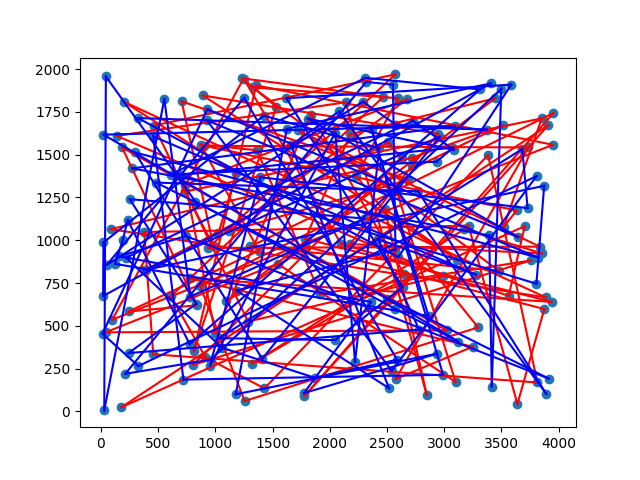
\includegraphics[width=\linewidth]{best_paths_constructions/kroA200/randomstart}
        \caption{kroA200, losowe rozwiązanie}
    \end{minipage}
    \hfill
    \begin{minipage}[t]{0.45\textwidth}
        \centering
        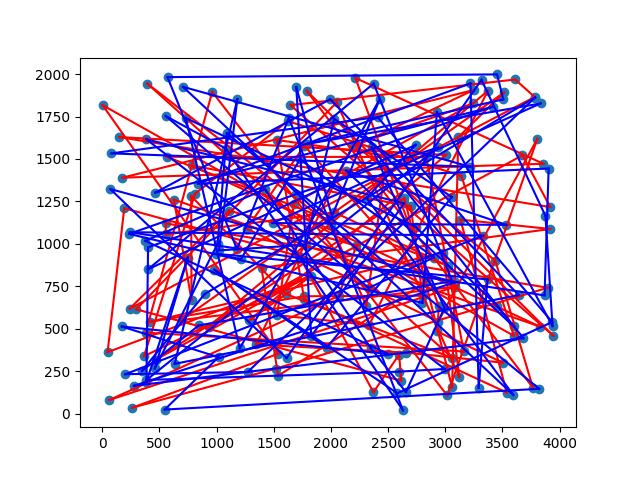
\includegraphics[width=\linewidth]{best_paths_constructions/kroB200/randomstart}
        \caption{kroB200, losowe rozwiązanie}
    \end{minipage}\label{fig:figure33}
\end{figure}


\subsubsection{split-lab1}
\begin{figure}[H]
    \begin{minipage}[t]{0.45\textwidth}
        \centering
        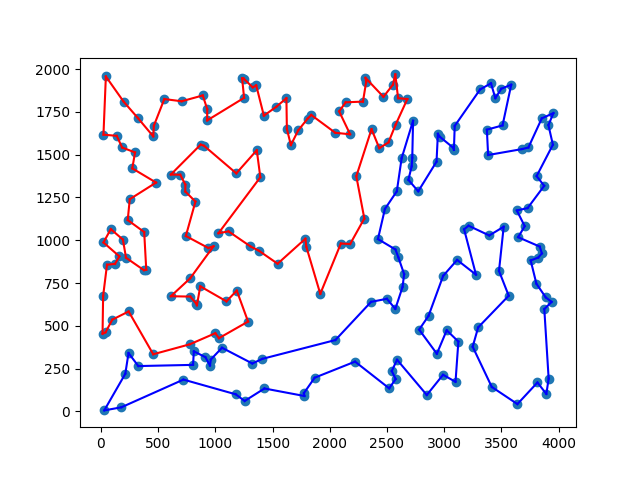
\includegraphics[width=\linewidth]{best_paths_constructions/kroA200/split_paths_regret_TSP}
        \caption{kroA200, heurystyka konstukcyjna z podziałem}
    \end{minipage}
    \hfill
    \begin{minipage}[t]{0.45\textwidth}
        \centering
        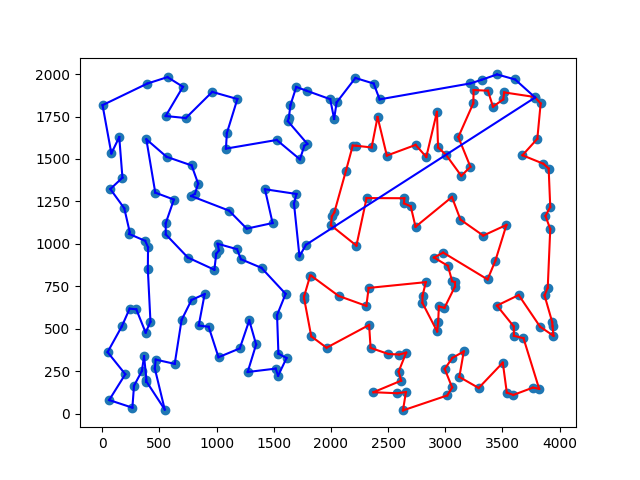
\includegraphics[width=\linewidth]{best_paths_constructions/kroB200/split_paths_regret_TSP}
        \caption{kroB200, heurystyka konstukcyjna z podziałem}
    \end{minipage}\label{fig:figure34}
\end{figure}


\subsubsection{spectral-split}
\begin{figure}[H]
    \begin{minipage}[t]{0.45\textwidth}
        \centering
        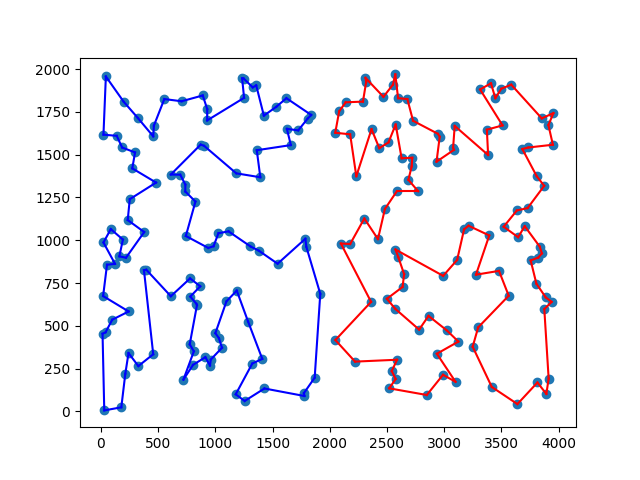
\includegraphics[width=\linewidth]{best_paths_constructions/kroA200/spectral_split_two_regret}
        \caption{kroA200, heurystyka konstukcyjna z podziałem spektralnym}
    \end{minipage}
    \hfill
    \begin{minipage}[t]{0.45\textwidth}
        \centering
        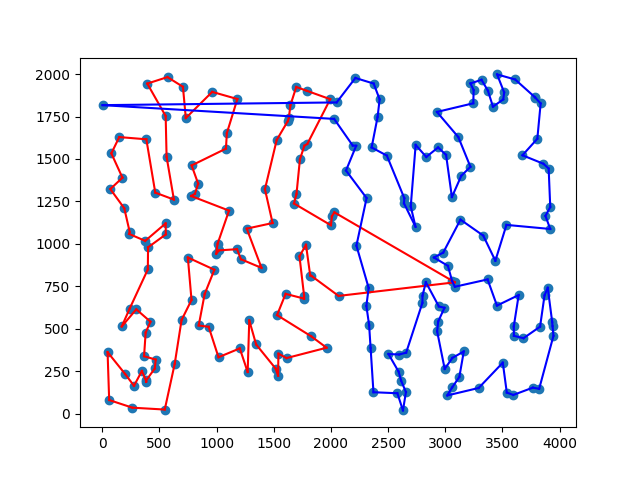
\includegraphics[width=\linewidth]{best_paths_constructions/kroB200/spectral_split_two_regret}
        \caption{kroB200, heurystyka konstukcyjna z podziałem spektralnym}
    \end{minipage}\label{fig:figure35}
\end{figure}

\subsubsection{MSLS}
\begin{figure}[H]
    \begin{minipage}[t]{0.45\textwidth}
        \centering
        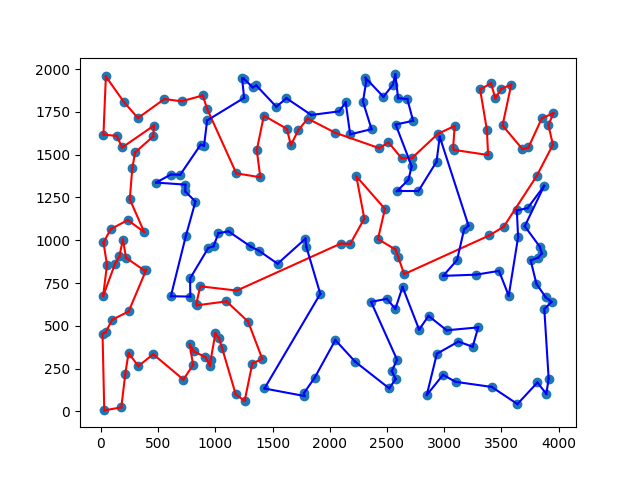
\includegraphics[width=\linewidth]{best_paths/kroA200/MSLS}
        \caption{kroA200, losowy start}
    \end{minipage}
    \hfill
    \begin{minipage}[t]{0.45\textwidth}
        \centering
        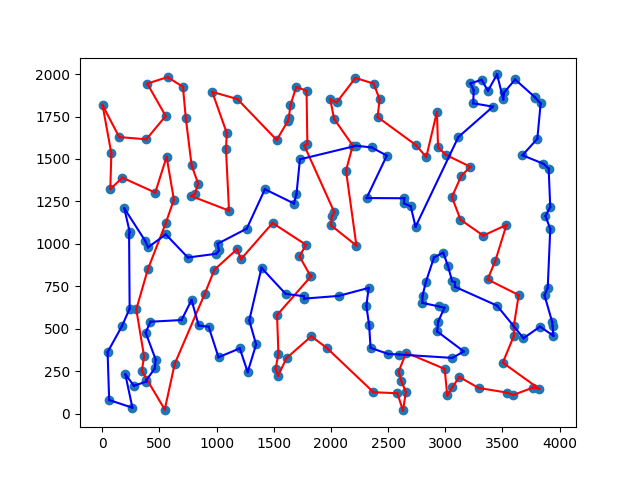
\includegraphics[width=\linewidth]{best_paths/kroB200/MSLS}
        \caption{kroB200, losowy start}
    \end{minipage}\label{fig:figure3}
\end{figure}

\subsubsection{ILS}

\begin{figure}[H]
    \begin{minipage}[t]{0.45\textwidth}
        \centering
        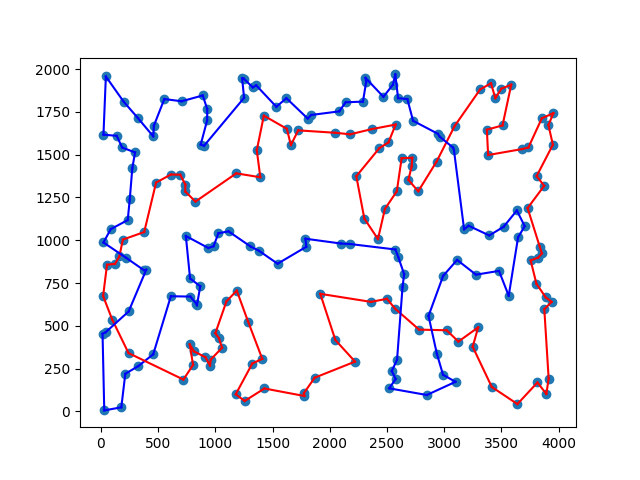
\includegraphics[width=\linewidth]{best_paths/kroA200/ILS}
        \caption{kroA200, losowy start}
    \end{minipage}
    \hfill
    \begin{minipage}[t]{0.45\textwidth}
        \centering
        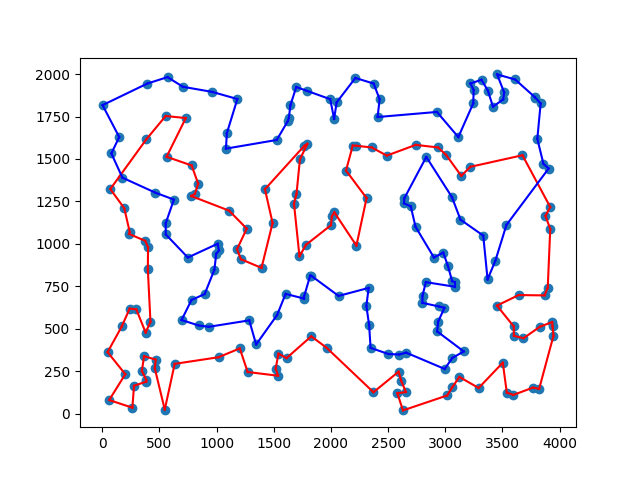
\includegraphics[width=\linewidth]{best_paths/kroB200/ILS}
        \caption{kroB200, losowy start}
    \end{minipage}\label{fig:figure1}
\end{figure}

\subsubsection{LNS}

\begin{figure}[H]
    \begin{minipage}[t]{0.45\textwidth}
        \centering
        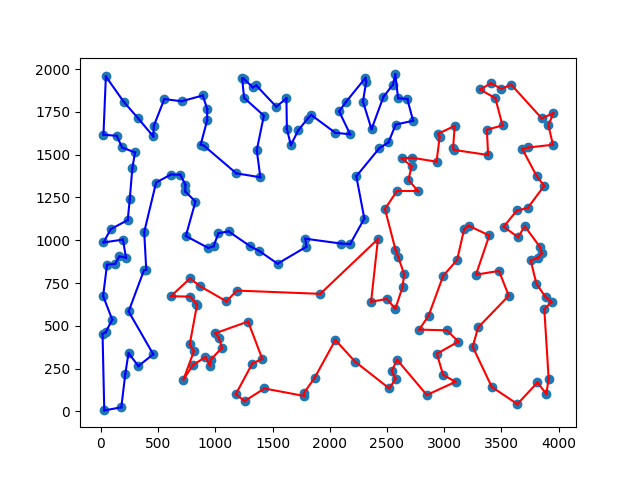
\includegraphics[width=\linewidth]{best_paths/kroA200/LNS}
        \caption{kroA200, losowy start}
    \end{minipage}
    \hfill
    \begin{minipage}[t]{0.45\textwidth}
        \centering
        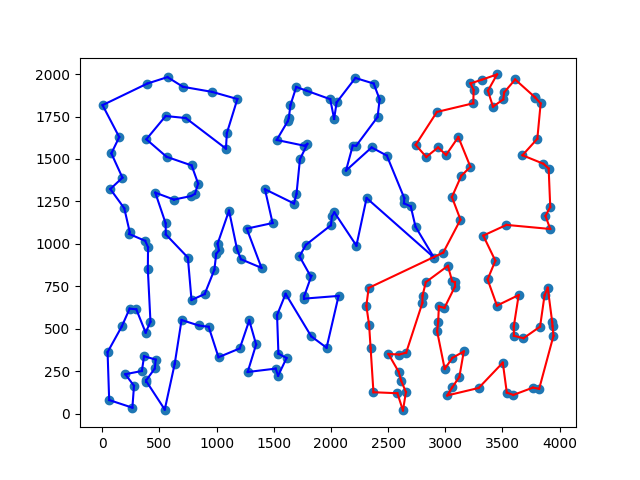
\includegraphics[width=\linewidth]{best_paths/kroB200/LNS}
        \caption{kroB200, losowy start}
    \end{minipage}\label{fig:figure2}
\end{figure}

\subsubsection{HAE z mutacją i lokalnym przeszukiwaniem}

\begin{figure}[H]
    \begin{minipage}[t]{0.45\textwidth}
        \centering
        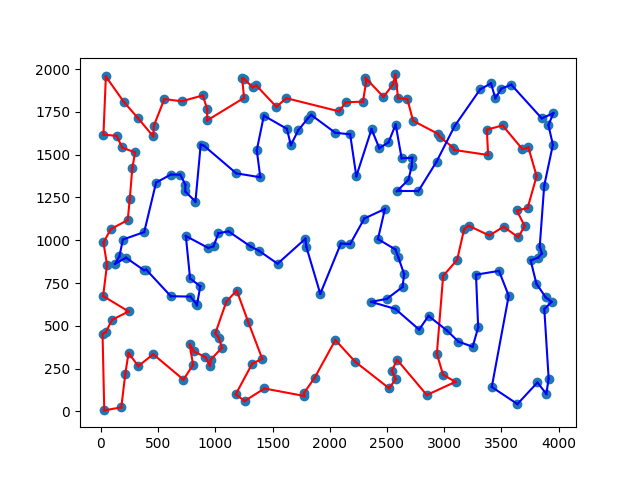
\includegraphics[width=\linewidth]{best_paths/kroA200/HAE+Mutation+LS}
        \caption{kroA200, losowy start}
    \end{minipage}
    \hfill
    \begin{minipage}[t]{0.45\textwidth}
        \centering
        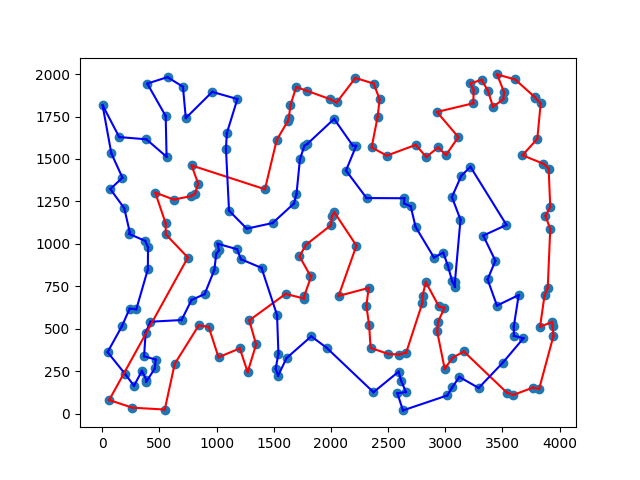
\includegraphics[width=\linewidth]{best_paths/kroB200/HAE+Mutation+LS}
        \caption{kroB200, losowy start}
    \end{minipage}\label{fig:figure8}
\end{figure}

\subsection{Wnioski}\label{subsec:wnioski}
Zaprojektowana przez nas heurystyka konstrukcyjna wykazuje się niebywałą szybkością i jest świetną opcją jeśli zależy nam na czasie.
W przypadku, gdy dążymy do jak najdokładniejszych rozwiązań nie zważając tak na czas, to połączenie jej z TODO algorytmem TODO robi TODO


\section{Testy globalnej wypukłości}\label{sec:testy-globalnej-wypukosci}

Wygenerowaliśmy 1000 lokalnych optimów dla każdej z analizowanych instancji problemu, za pomocą lokalnego przeszukiwania w wersji zachłannej z losowych rozwiązań początkowych.
Obliczyliśmy podobieństwa każdego lokalnego optimum do rozwiązania referencyjnego (bardzo dobrego) oraz średnie podobieństwo do pozostałych lokalnych optimów.
Korzystamy z dwóch miar podobieństwa: Liczby par wierzchołków przydzielonych do tego samego cyklu w obu rozwiązaniach oraz z liczby wspólnych krawędzi w rozwiązaniach.

\subsection{Wyniki dla instancji kroA200}\label{subsec:wyniki-dla-instancji-kroa200}

\begin{figure}[H]
    \begin{minipage}[t]{0.45\textwidth}
        \centering
        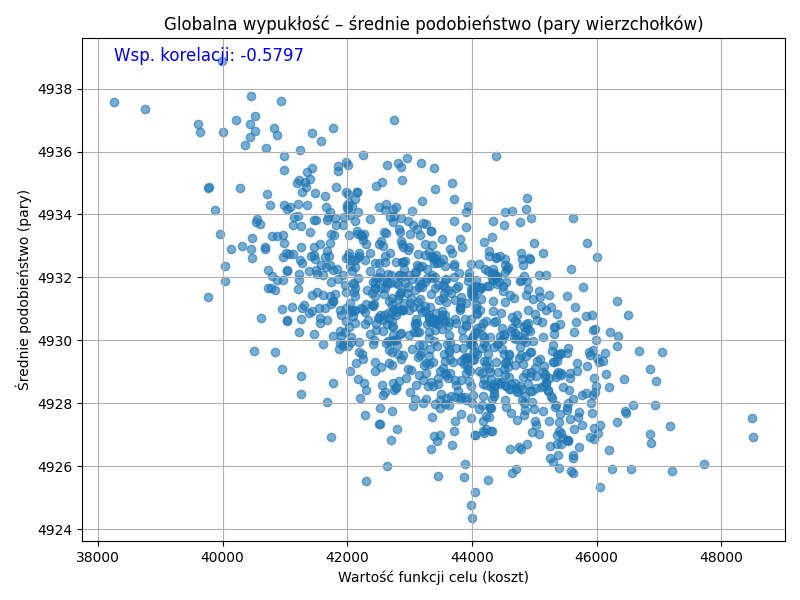
\includegraphics[width=\linewidth]{wypuklosci/podobienstwo-parami-kroA}
        \caption{podobieństwo parami - kroA}
    \end{minipage}
    \hfill
    \begin{minipage}[t]{0.45\textwidth}
        \centering
        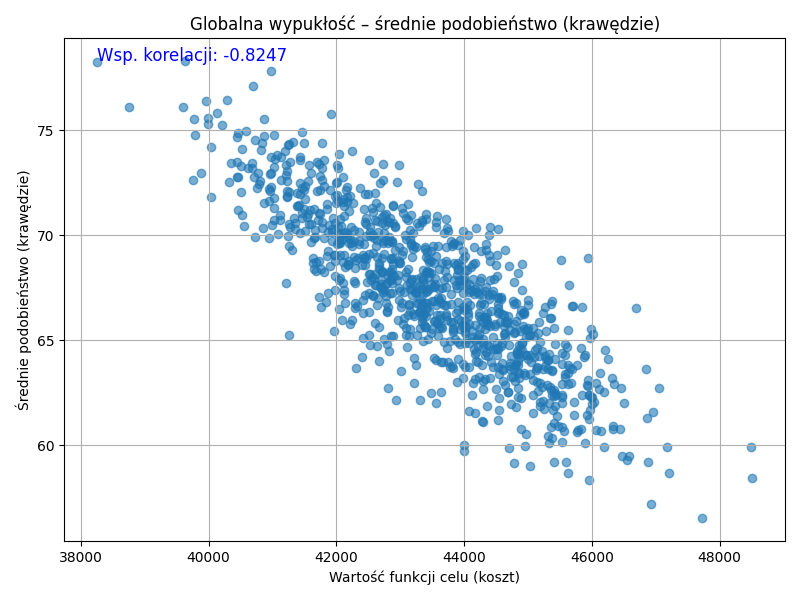
\includegraphics[width=\linewidth]{wypuklosci/podobienstwo-krawedziami-kroA}
        \caption{podobieństwo krawedziami - kroA}
    \end{minipage}\label{fig:figure11}
\end{figure}

\begin{figure}[H]
    \begin{minipage}[t]{0.45\textwidth}
        \centering
        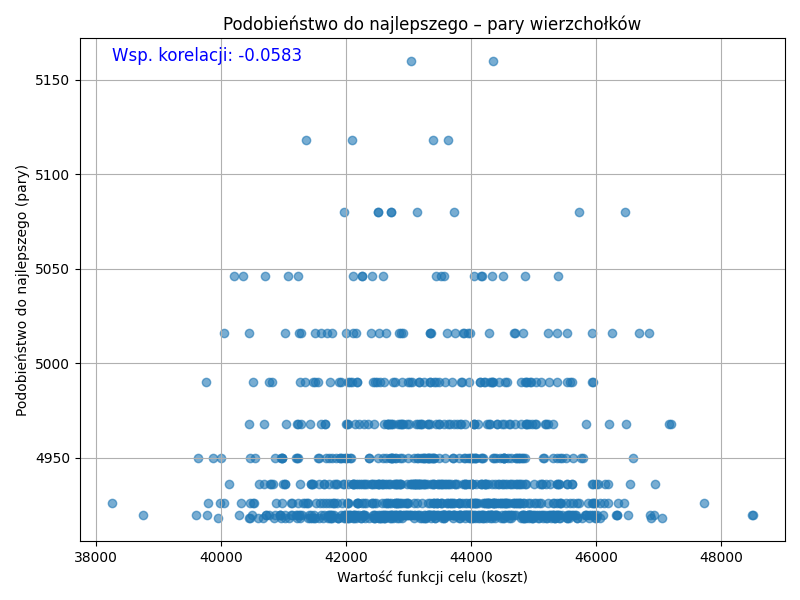
\includegraphics[width=\linewidth]{wypuklosci/podobienstwo-naj-parami-kroA}
        \caption{podobieństwo parami do najlepszego- kroA}
    \end{minipage}
    \hfill
    \begin{minipage}[t]{0.45\textwidth}
        \centering
        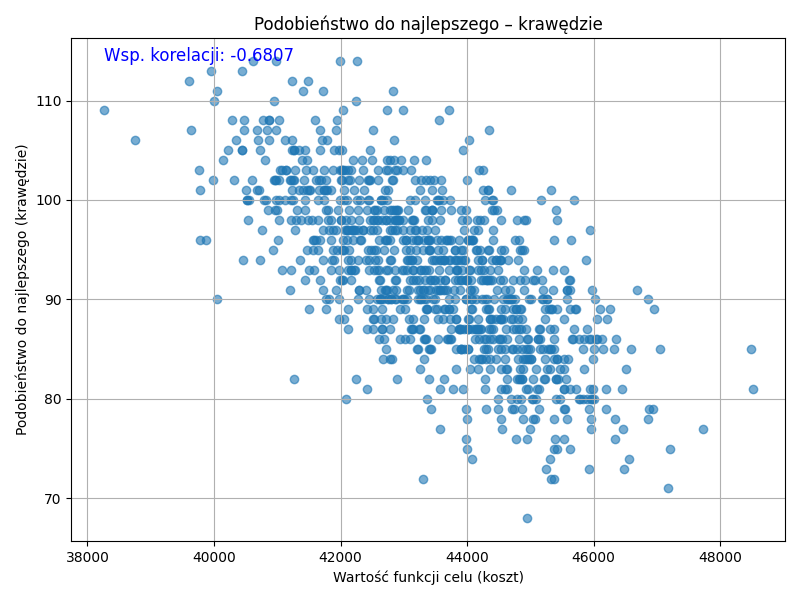
\includegraphics[width=\linewidth]{wypuklosci/podobienstwo-naj-krawedziami-kroA}
        \caption{podobieństwo krawedziami do najlepszego- kroA}
    \end{minipage}\label{fig:figure12}
\end{figure}


\subsection{Wyniki dla instancji kroB200}\label{subsec:wyniki-dla-instancji-krob200}

\begin{figure}[H]
    \begin{minipage}[t]{0.45\textwidth}
        \centering
        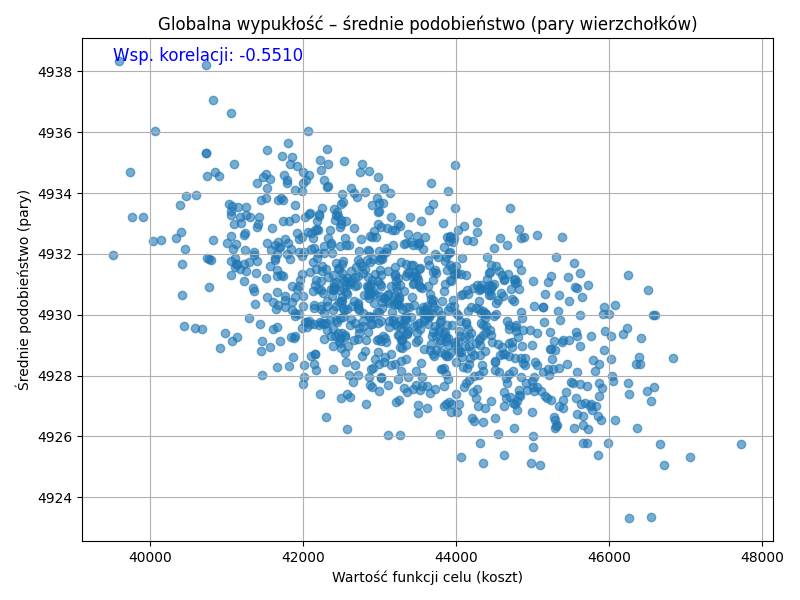
\includegraphics[width=\linewidth]{wypuklosci/podobienstwo-parami-kroB}
        \caption{podobieństwo parami - kroB}
    \end{minipage}
    \hfill
    \begin{minipage}[t]{0.45\textwidth}
        \centering
        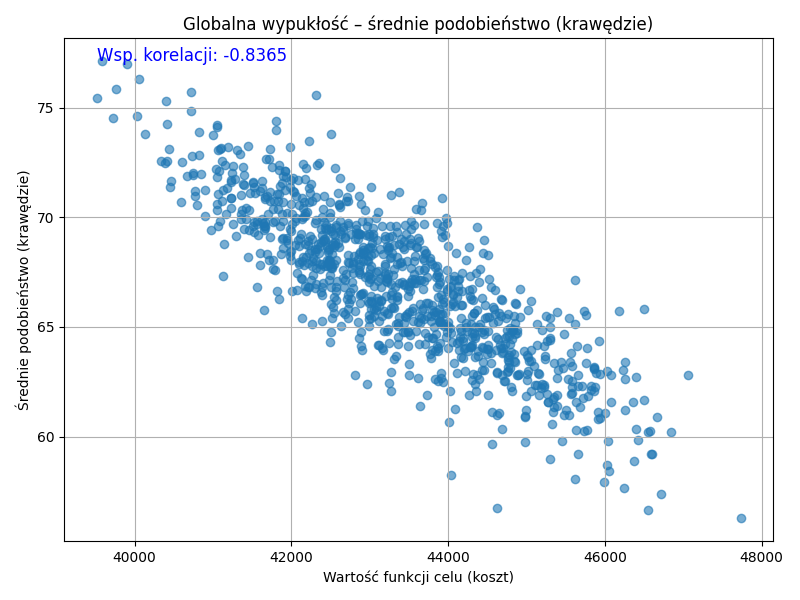
\includegraphics[width=\linewidth]{wypuklosci/podobienstwo-krawedziami-kroB}
        \caption{podobieństwo krawedziami - kroB}
    \end{minipage}\label{fig:figure13}
\end{figure}

\begin{figure}[H]
    \begin{minipage}[t]{0.45\textwidth}
        \centering
        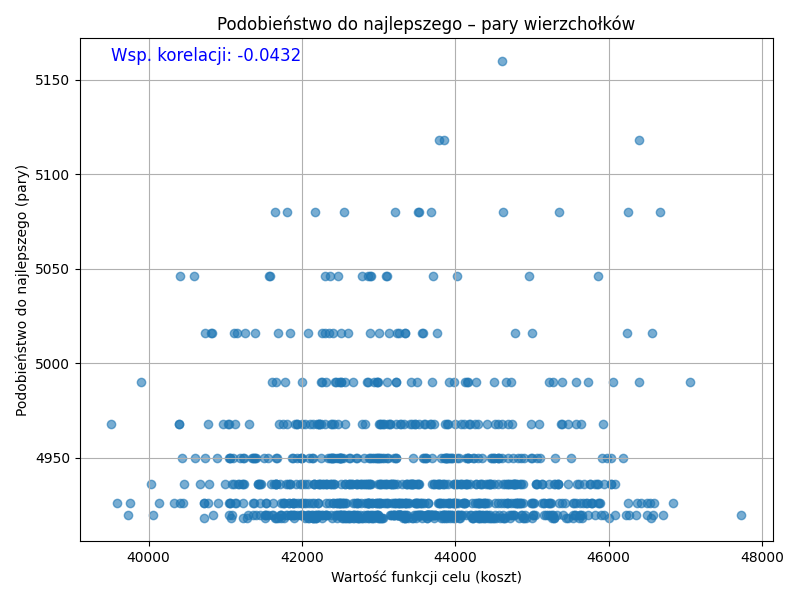
\includegraphics[width=\linewidth]{wypuklosci/podobienstwo-naj-parami-kroB}
        \caption{podobieństwo parami do najlepszego- kroB}
    \end{minipage}
    \hfill
    \begin{minipage}[t]{0.45\textwidth}
        \centering
        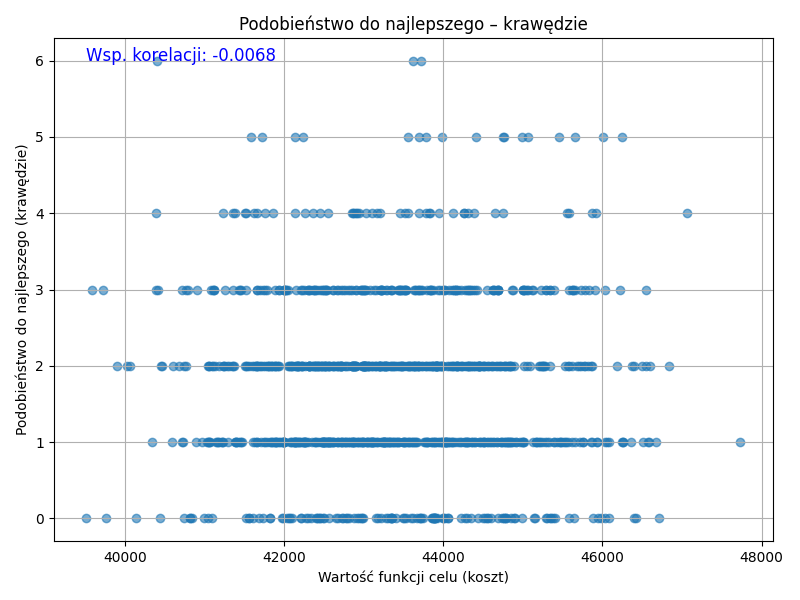
\includegraphics[width=\linewidth]{wypuklosci/podobienstwo-naj-krawedziami-kroB}
        \caption{podobieństwo krawedziami do najlepszego- kroB}
    \end{minipage}\label{fig:figure14}
\end{figure}


\subsection{Wnioski}\label{subsec:wnioski-wypuklosci}

Na podstawie powyższych eksperymentów można stwierdzić że funkcja wykazuje cechy globalnej wypukłości.
Przede wszystkim, przemawia za tym silna ujemna korelacja między wartością funkcji celu, a średnim podobieństwem do innych lokalnych minimów.
Miara podobieństwa oparta na krawędziach zdaje się lepiej oddawać strukturę przestrzeni rozwiązań, niż ta oparta na parach wierzchołków (patrząc stricte na siłę korelacji).
W ogólności, eksperyment pokazał że dobre rozwiązania są do siebie podobne, co jest zgodne z definicją globalnej wypukłości - choć nie implikuje że wszystkie podobne rozwiązania będą dobre.


\section{Link do repozytorium}\label{sec:link-do-repo}
Kod źródłowy w repozytorium GitHub dostępny pod linkiem:
\href{https://github.com/KotZPolibudy/PUT_IMO/tree/main/Lab6%20-%20Testy%20wypuklosci%20i%20wlasna%20metoda}{Repozytorium}.

\end{document}
